% !TEX root = ../paper.tex
\section{Discussion}
\label{sec:discussion}

When looking at the results on the effect of the four techniques, \pinch, \tilt, \swipe and \throw, as well as the two grid sizes, large and small, on the time per target, the results tell a rather interesting story. An overview of the results can be seen in \Cref{fig:timeResults}.

\ref{fig:timeResults}. 
\begin{figure}[H]
	{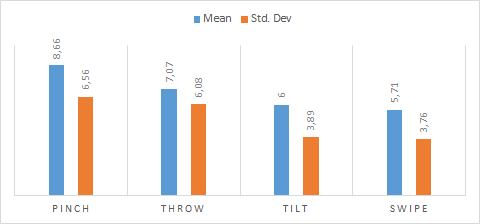
\includegraphics[width = 1\columnwidth ]{images/timeResults.png}} 
	\caption{
		Overview of the mean and standard deviation of each technique.
	}
	\label{fig:timeResults}
\end{figure}

There was a significant difference between all techniques, with the exception of \swipe and \tilt. These were the two one handed techniques that were created. The range of movement needed in order to activate these two techniques was rather limited, the full motion could be achieved quite quickly and is quite similar for both of them.  This is why they are not statistically different from each other. \swipe and \tilt, are on average, at least a second faster then the other two. Their standard deviation are also smaller, which means that users were more consistent, with regards to how long it took to hit each target, with these two techniques. 

Looking at the two other techniques, \pinch and \throw, their times also reflect the range of motion needed in order to activate each technique. \pinch requires the user to pinch the shape on their phone, lift their hand up, direct it on the screen, and then finally let go. This can be seen in its mean, where it takes almost 1.59 seconds longer to perform than the seconds longest technique, \throw. \throw also requires a considerable range of motion in order to activate: point with one arm, select the shape on the phone on the other, bring your arm back and then finally swing it forward. Both two handed techniques take significantly longer time to perform than the one handed counter-parts. 


\subsection{Limitations}

The intention with the \tilt technique was that the users would point and tilt with the phone, but because of our implementation, it was possible for users to point with one hand and tilt the phone with the other.
Again, because of our implementation of the \swipe technique, users were able to point with one hand and swipe with the other.